
\section{Intégration de moteurs dans le SI}

\begin{frame}{Moteurs de recherche}
  Moteurs libres
  \begin{redbullet}
    \item Apache Solr (Lucene)
    \item {\color{red}ElasticSearch (Lucene)}
    \item Sphinx
    \item Xapian
  \end{redbullet}
  \medskip
  Moteurs commerciaux
  \begin{redbullet}
    \item Google Search Appliance
    \item Exalead, Qwant
    \item Amazon CloudSearch
    \item Microsoft Azure Search, Bing
  \end{redbullet}
\end{frame} % ending frame Moteurs de recherche

\begin{frame}{Bases documentaires et moteur de recherche}
  \begin{center}
    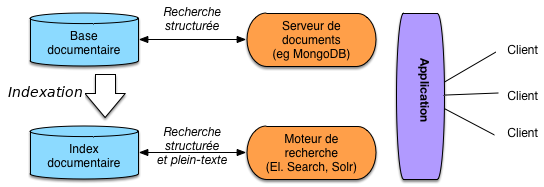
\includegraphics[width=13cm]{../figures/archi-ri2.png}
  \end{center}
\end{frame}

\begin{frame}{Bases documentaires et moteur de recherche}
Un scénario typique :
\begin{redbullet}
  \item une recherche par mot-clé dans un site
  \item Les données du site sont gérées classiquement par une base documentaire
    (MySQL, Postgres, MongoDB)
  \item On extrait de la base tous les textes à \alert{indexer} et on en fait
    des documents JSON, transmis au moteur de recherche
  \item Ce dernier se charge alors de répondre quand un utilisateur emploie un champ de recherche.
\end{redbullet}
\end{frame} % ending frame 


\begin{frame}{Bases documentaires et moteur de recherche}

Un système comme ElasticSearch est consacré à la \alert{recherche},
    c'est-à-dire la lecture la plus efficace possible de documents.

\vfill

Il s'appuie pour cela sur des structures compactes, compressées,
    optimisées (les \alert{index inversés}) 

\vfill

Ce n'est pas (pas forcément) un très bon outil pour les autres fonctionnalités
    d'une base de données :
    \begin{redbullet}
      \item Le stockage par exemple n'est ni aussi robuste ni aussi stable.
      \item Mises à jour coûteuses et asynchrones
    \end{redbullet}

\end{frame} % ending frame 

\begin{frame}{Présentation d'Elasticsearch}
  Elasticsearch est un moteur de recherche basé sur Lucene
  \begin{redbullet}
    \item grande communauté d'utilisateurs
    \item open source, profite de la recherche dans le domaine sur Lucene
    \item utilisé par de grands opérateurs du Web sur des collections immenses
  \end{redbullet}
  \medskip
  En fait, plusieurs composants dont :
  \begin{redbullet}
    \item Logstash, l'ETL, pour extraire, transformer et charger les données
    \item ElasticSearch, le moteur lui-même
    \item Kibana, pour produire des tableaux de bords de surveillance
  \end{redbullet}
\end{frame}


\begin{frame}[fragile]{Interrogation}
  \begin{redbullet}
    \item ElasticSearch s’appuie sur le système d’indexation \textbf{Lucene},
      dont le rôle est essentiellement de créer les index inversés, et
      d’implanter les algorithmes de parcours brièvement introduits dans la
      session précédente. 

\item Lucene propose un langage de recherche basé sur des combinaisons de
  mot-clés, langage étendu et raffiné par ElasticSearch (cf plus tard)
\item La première méthode pour transmettre des recherches est de passer une
  expression en paramètre à l’URL :
\begin{minted}[frame=lines,
               baselinestretch=.9,
               fontsize=\footnotesize,
               framesep=2mm]{bash}
http://localhost:9200//nfe204/movies/_search?q=alien
http://localhost:9200/nfe204/movies/_search?q=alien,coppola
http://localhost:9200/nfe204/movies/_search?q=alien,coppola,1994
# utilisable dans l'interface ElasticVue, onglet Rest
\end{minted}

\end{redbullet}
\end{frame}

\begin{frame}[fragile]{la réponse d'ES}
	\begin{minted}[ baselinestretch=0.9, fontsize=\tiny, ]{bash}
{
  "took" : 1,
  "timed_out" : false,
  "_shards" : {
    "total" : 1,
    "successful" : 1,
    "failed" : 0
  },
  "hits" : {
    "total" : 1,
    "max_score" : 0.558217,
    "hits" : [ {
      "_index" : "nfe204",
      "_type" : "movies",
      "_id" : "movie:2",
      "_score" : 0.558217,
      "_source":{ "title": "Alien", "year": 1979, 
                  "genre": "Science-fiction",
                   "summary": "... ", 
                   "country": "USA", 
                   "director": "Ridley Scott", 
                   "actors": [ ["Sigourney Weaver"]   ] }
    } ]
  }
}

\end{minted} 
\end{frame} 


\begin{frame}[fragile]{Termes}

  \begin{redbullet}
    \item Notion de base : le {\bf terme}
    \item c'est un mot au sens usuel
    \item ou une séquence de mots entre apostrophes
  \end{redbullet}
\smallskip
On peut interroger un index avec :
\begin{minted}[frame=lines, baselinestretch=.9, fontsize=\footnotesize, framesep=2mm]{sql}
Neo apprend
\end{minted}
Puis :
\begin{minted}[frame=lines, baselinestretch=.9, fontsize=\footnotesize, framesep=2mm]{sql}
  "Neo apprend"
\end{minted}
\vfill
\begin{blocgauche}
  Première recherche : documents avec ``Neo'', ``apprend'' ou les deux
\end{blocgauche}

\end{frame}

\begin{frame}[fragile]{Termes (suite)}
  \begin{redbullet}
    \item la recherche d'un terme s'effectue toujours sur un champ. 
\item La syntaxe complète pour associer le champ et le terme est:
\begin{minted}[frame=lines,
               baselinestretch=.9,
               fontsize=\footnotesize,
               framesep=2mm]{sql}
  champ:terme
\end{minted}
\item si non précisé, c'est le champ par défaut qui est utilisé
\item pratique courante : concaténer toutes les chaînes de caractères en un
  champ ``\_all'' général, défini par défaut
\item Nos requêtes deviennent :
\begin{minted}[baselinestretch=.9,
               fontsize=\footnotesize,
               framesep=2mm]{sql}

               _all:Neo _all:apprend
\end{minted}
\item et 
\begin{minted}[baselinestretch=.9,
               fontsize=\footnotesize,
               framesep=2mm]{sql}
               _all:"Neo apprend"
\end{minted}
  \end{redbullet}
\end{frame}

\begin{frame}[fragile]{Termes (suite)}

  \begin{redbullet}
    \item Les valeurs des termes (dans la requête) et le texte indexé sont tous deux
soumis à des transformations spécifiées dans le schéma. 
\item Une transformation simple est de tout transcrire en minuscules. 
\begin{minted}[frame=lines,
               baselinestretch=.9,
               fontsize=\footnotesize,
               framesep=2mm]{sql}
              _all:"Neo APPREND"
\end{minted}
\item  Les transformations appliquées à la requête ET au texte indexé doivent être 
   cohérentes : si les termes sont transformés en majuscules, et le texte indexé en minuscules,
   on n'aura jamais de résultat!
  \end{redbullet}
\end{frame}

\begin{frame}[fragile]{Termes (suite)}
  On peut spécifier des termes (pas des séquences) incomplets
  \begin{redbullet}
      \setlength{\itemsep}{8pt}
    \item le '?' indique un caractère inconnu;  ``opti?al'' désigne ``optimal'', ``optical'', etc.
      
    \item le '*' indique n'importe quelle séquence de caractères; 
      ``opti*'' pour toute chaîne commençant par ``opti''
    \item Approximation avec $\sim$: rechercher ``optimal`` et ``optimal$\sim$`` (0 et 1 résultat, ''optical'')
    
       La similarité est évaluée par une distance d'édition 
      (nb opérations pour passer de ``optimal'' à ``optical'')
  
    \item Les intervalles sont exprimés avec  $[ ]$ (bornes comprises) ou  \{ \} bornes exclues
  \end{redbullet}
\begin{minted}[frame=lines,
               baselinestretch=.9,
               fontsize=\footnotesize,
               framesep=2mm]{sql}
    year:[1984 TO 2010]
\end{minted}
\end{frame}

\begin{frame}[fragile]{Requêtes Booléennes}

  \begin{redbullet}
    \item Les critères peuvent être combinés avec des \alert{opérateurs
      Booléens} :\\
      \variable{AND}, \variable{OR} et \variable{NOT}
    \item Attention : majuscules
  \end{redbullet}
\begin{minted}[frame=lines,
               baselinestretch=.9,
               fontsize=\footnotesize,
               framesep=2mm]{sql}
year:[1990 TO 2005] OR title:M*
year:[1990 TO 2005] AND NOT title:M*
\end{minted}
   
\begin{redbullet}
  \item Par défaut, c'est un \variable{OR} qui est appliqué
  \item Recherche sur plusieurs critères ramène l'union des résultats sur chaque
    critère pris individuellement
  %\item La requête suivante recherche les produits Dell {\bf ou} dont la popularité est
%égale à 6 :
%\begin{minted}[frame=lines,
               %baselinestretch=.9,
               %fontsize=\footnotesize,
               %framesep=2mm]{sql}
    %%popularity:6  manu:Dell
%\end{minted}
\end{redbullet}
\end{frame}

\begin{frame}[fragile]{Requêtes structurées}

On fournit un document décrivant la requête en la \textit{postant}  
(méthode \texttt{POST}):

\vfill

\begin{minted}[ baselinestretch=0.9]{bash}
	{
    	"query": {
      		"match": {
        		"title": "Star Wars"
      		}
  		}
   	}
\end{minted}

\vfill

Un premier pas vers une interrogation plus structurée.

\end{frame}

\begin{frame}[fragile]{Choix des champs et du résultat}

On peut ajouter des spécifications dans la requête.

\vfill

\begin{minted}[ baselinestretch=0.9]{bash}
	{
    	"query": {
      		"match": {
        		"title": "Star Wars"
      		}
  		},
  		"fields": ["title"],
  		"_source": false
   	}
\end{minted}

\end{frame}

\begin{frame}[fragile]{Effectuer des recherches approchées}

\begin{minted}[ baselinestretch=0.9]{bash}
	{
	  "query": {
	     "fuzzy": {
      		"title": {
        		"value": "matrice"
    	  	}
    	  }
  		},
  	 "fields": ["title"],
	 "_source": false
	}
\end{minted}

\end{frame}


\begin{frame}[fragile]{Recherches par intervalle}

\begin{minted}[ baselinestretch=0.9]{bash}
	{
  		"query": {
		    "range": {
		      "year": {"gte": 2010, "lte": 2020}
    		}
  		},
  		"fields": ["title", "year"],
  		"_source": false
	}
\end{minted}

\end{frame}





%\begin{frame}[fragile]{Opérateur $+$, classement}
  %\begin{redbullet}
    %\item préfixe d'un nom de champ, il indique que la valeur du champ {\bf doit}
      %être égale au terme
    %\item il existe également un opérateur $-$, équivalent au \variable{NOT}
    %\item recherche des documents dont la popularité est 6 (obligatoire) et qui peuvent
%être produits par Dell ou un autre constructeur 
%\begin{minted}[frame=lines,
               %baselinestretch=.9,
               %fontsize=\footnotesize,
               %framesep=2mm]{sql}
    %%+popularity:6  manu:Dell
%\end{minted}
%\item différence avec ce qui précède : le {\bf classement} du moteur
%\item illustre la différence entre recherche d'information et interrogation
  %de bases de données
  %\end{redbullet}
  %\bigskip
  %Interpréter un classement est parfois délicat :\\
%\begin{minted}[frame=lines,
               %baselinestretch=.9,
               %fontsize=\footnotesize,
               %framesep=2mm]{sql}
    %%+popularity:6  cat:electronics

    %%+popularity:6  -manu:Dell

%\end{minted}
%\end{frame}


\begin{frame}[fragile]{En conclusion}


Ce qui précère constitue l'essentiel des opérations d'interrogation avec un moteur
de recherche.

  \begin{redbullet}
    \item On est loin de la finesse d'interrogation d'un langage comme SQL.
    
    \item On fait peu mais on fait bien: systèmes extrêmement efficaces, même pour
        de très grands volumes. 
  \end{redbullet}

\vfill

\alert{Surtout}, deux différences essentielles:

 \begin{redbullet}
    \item Le système permet des recherches \alert{approchées}: on trouve tous les documents "proches de" la requête
    \item Le résultat peut être \alert{ordonné} par pertinence décroissante.
  \end{redbullet}

\vfill

Comme ça marche? Voir la suite...
\end{frame}

